\documentclass[11pt,a4paper]{article}
\usepackage[T1]{fontenc}
\usepackage[utf8]{inputenc}
\usepackage{lmodern}
\usepackage[margin=2.3cm]{geometry}
\usepackage{microtype}
\usepackage{graphicx}
\usepackage{booktabs}
\usepackage[font=small,labelfont=bf]{caption}
\usepackage[hidelinks]{hyperref}
\usepackage{enumitem}
\usepackage{float}
\setlist{nosep,leftmargin=*}
\graphicspath{{../figures/}}
\newcommand{\x}{$\times$}

\title{Accelerating BERT-base training on a single A100\\[4pt]
\large HPC Tools, Lab AI: deliverable 1 (BASELINE)}
\author{Nicolás Aller Ponte}
\date{30 September 2026}

\begin{document}
\maketitle

\begin{abstract}
\noindent
We fine-tune BERT-base for question answering on SQuAD v1.1 on one NVIDIA A100 of FinisTerrae III
and apply the single-GPU optimizations of the course one at a time, profiling each of them.
Two epochs take 45.8 minutes in the FP32 baseline and 7.2 minutes once optimized, a 6.4\x{}
speedup, while F1 drops by one point (87.97 to 86.97). Precision is the decisive lever; the
remaining optimizations each remove the bottleneck exposed by the previous one.
\end{abstract}

\section{Setup and method}

The model is \texttt{google-bert/bert-base-uncased} (109\,M parameters), trained for 2 epochs with
AdamW (learning rate $3\cdot10^{-5}$, 10\,\% linear warmup, then linear decay) on 88,492
training windows of 384 tokens. All runs use one A100-PCIE-40GB and 32 CPU cores, with
PyTorch 2.11 built for CUDA 12.8.

\begin{itemize}
  \item \textbf{Throughput} is measured over 100 steps after a warmup of 30 steps (60 with
        \texttt{torch.compile}), between two \texttt{torch.cuda.synchronize()} calls.
  \item Each configuration runs \textbf{three times}; we report the median and the range.
  \item \texttt{torch.profiler} records five steps per configuration. We report the \emph{share}
        of GPU time per kernel group: shares are comparable across configurations, whereas
        absolute times are not, since the profiled steps are the first ones of each run.
  \item The baseline is true FP32 (TF32 disabled), and quality is measured with the official
        SQuAD exact match and F1 on the full validation set.
\end{itemize}

\section{Deployment on FinisTerrae III}

Most of the effort went into running the code correctly on the cluster (Table~\ref{tab:deploy}).

\begin{table}[H]
\centering\small
\caption{Deployment issues and their solutions.}
\label{tab:deploy}
\begin{tabular}{p{7.4cm}p{7.4cm}}
\toprule
Issue & Solution \\
\midrule
The default PyTorch wheel targets CUDA 13; the A100 driver (570.86.15) supports up to 12.8 &
Install PyTorch from the CUDA 12.8 index \\
\texttt{python/3.10.10} is not available & \texttt{module load cesga/2020 python/3.10.8} \\
A GPU job with 4 cores is rejected & Exactly 32 cores per A100 \\
\texttt{\$HOME} quota is 20\,GB & Virtual environment and Hugging Face cache in \texttt{\$STORE} \\
Tokenizing in the training job would count as training time & A separate CPU job tokenizes once \\
Long jobs queue longer & Jobs under 6\,h run in the high-priority \texttt{short} QoS \\
\bottomrule
\end{tabular}
\end{table}

\section{Results}

\subsection{One optimization at a time}

\begin{figure}[H]
\centering
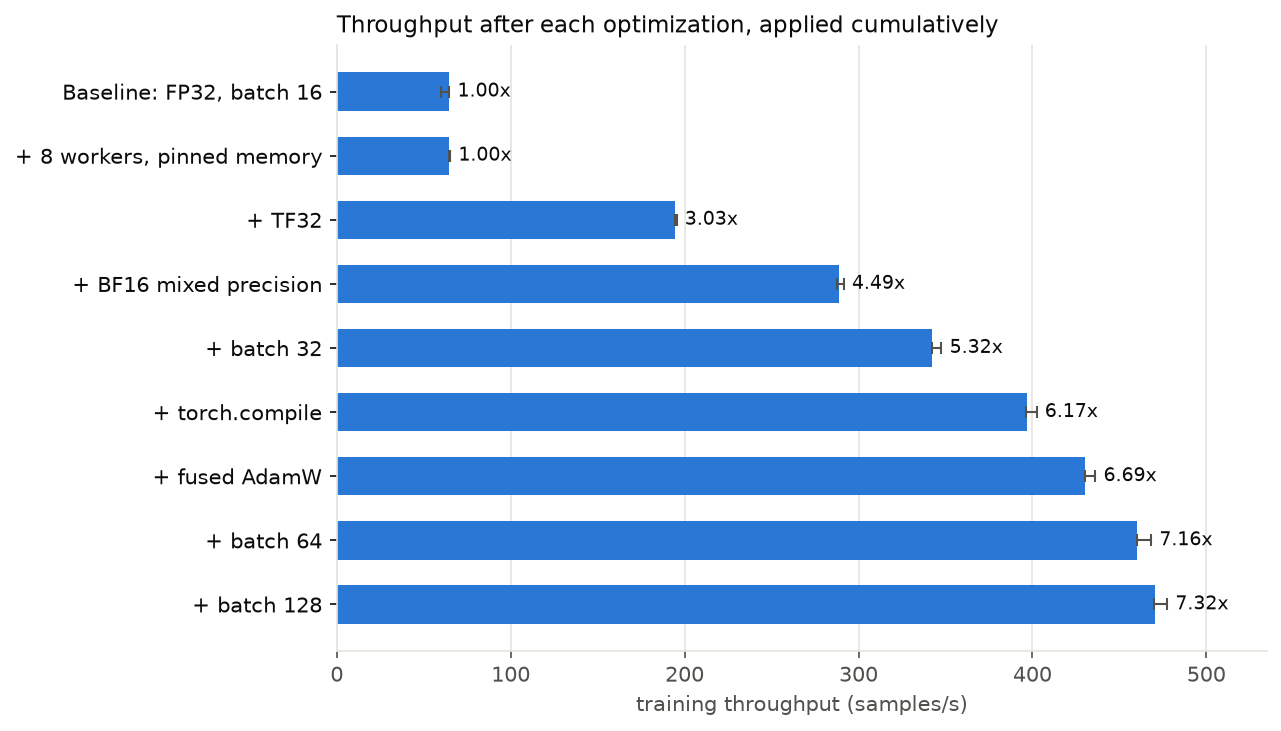
\includegraphics[width=0.8\linewidth]{throughput.png}
\caption{Training throughput after each cumulative optimization. Bars show the median of three
runs and whiskers the range; labels give the speedup over the baseline.}
\label{fig:throughput}
\end{figure}

\begin{table}[H]
\centering\small
\caption{Throughput and peak memory of each step (median and range of three runs).}
\label{tab:steps}
\begin{tabular}{rlrrr}
\toprule
Step & Change & Samples/s [range] & Speedup & Memory \\
\midrule
0 & Baseline: FP32, batch 16, no workers & 64.3 [60.0, 64.7] & 1.00\x & 5.3\,GB \\
1 & + 8 workers, pinned memory & 64.4 [64.4, 65.2] & 1.00\x & 5.3\,GB \\
2 & + TF32 & 194.6 [194.6, 195.4] & 3.03\x & 5.3\,GB \\
3 & + BF16 mixed precision & 289.0 [287.5, 291.5] & 4.49\x & 4.1\,GB \\
4 & + batch 32 & 342.2 [342.2, 347.7] & 5.32\x & 6.6\,GB \\
5 & + \texttt{torch.compile} & 397.0 [396.1, 402.4] & 6.17\x & 6.0\,GB \\
6 & + fused AdamW & 430.1 [430.0, 436.2] & 6.69\x & 6.0\,GB \\
7 & + batch 64 & 460.2 [460.0, 468.3] & 7.16\x & 10.4\,GB \\
8 & + batch 128 & 470.4 [470.2, 477.5] & 7.32\x & 19.3\,GB \\
\bottomrule
\end{tabular}
\end{table}

\subsection{Where the GPU time goes}

\begin{figure}[H]
\centering
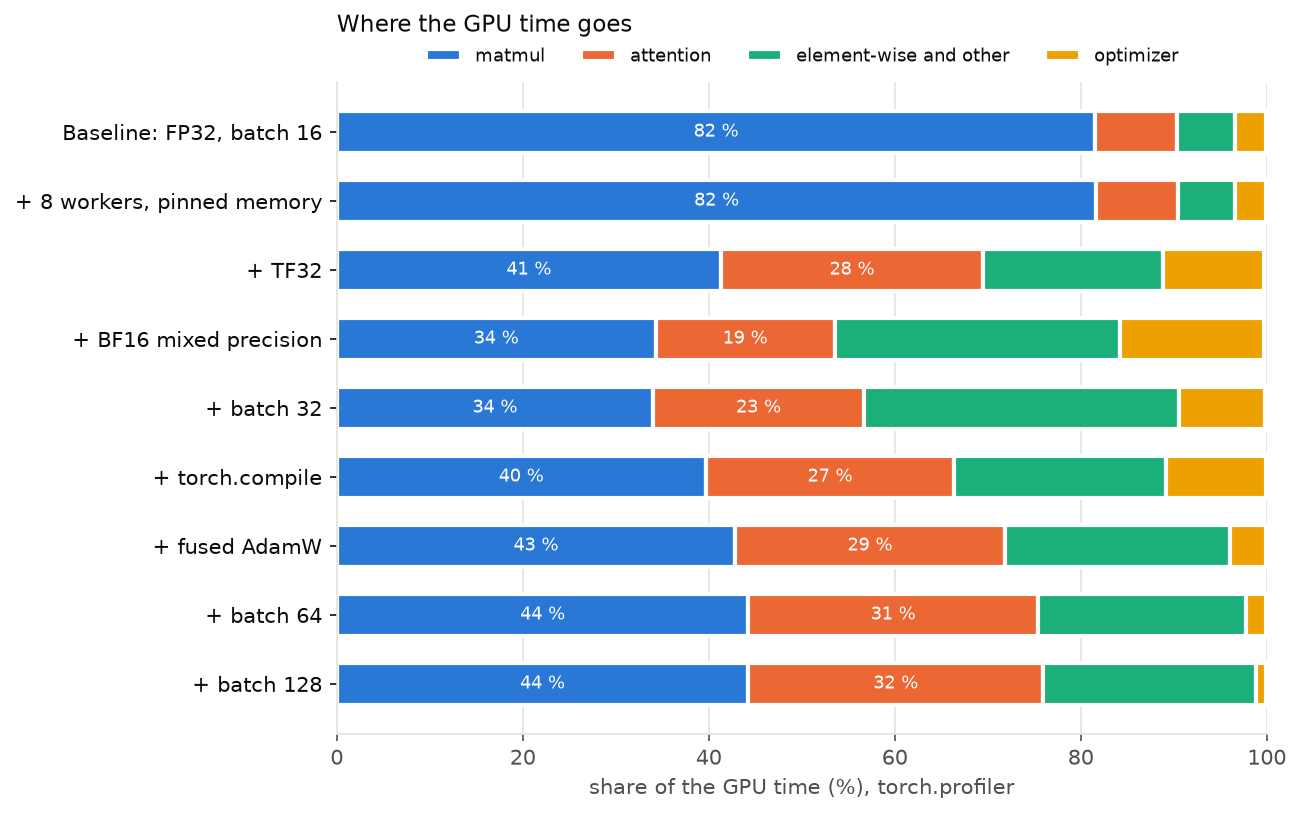
\includegraphics[width=0.8\linewidth]{profile.png}
\caption{Share of GPU time per kernel group, from the profiler traces. Kernels launched inside
the optimizer step are counted as optimizer. Memory copies stay below 0.5\,\%.}
\label{fig:profile}
\end{figure}

\subsection{Full training}

\begin{figure}[H]
\centering
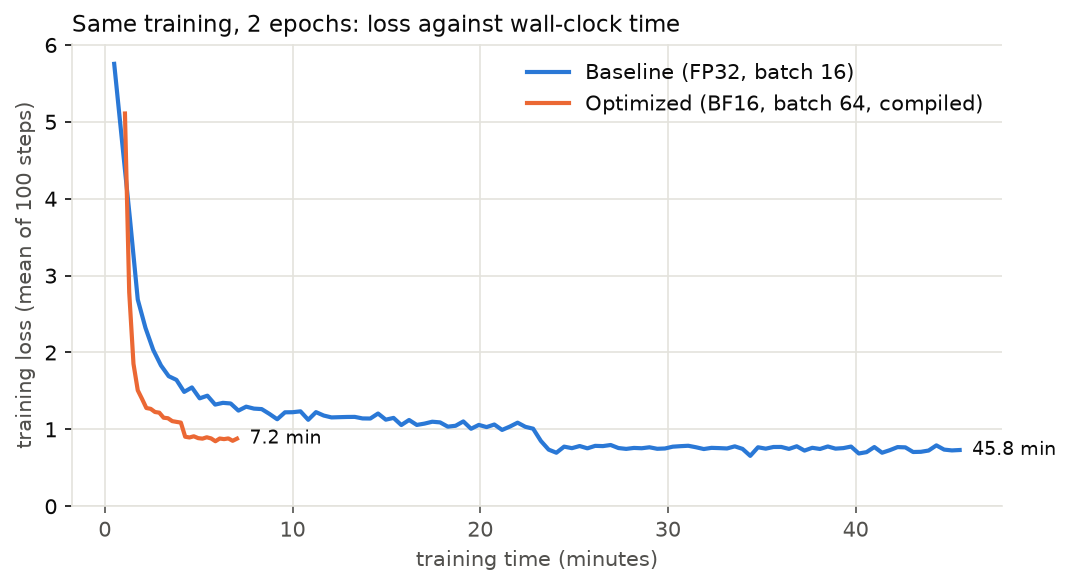
\includegraphics[width=0.74\linewidth]{loss.png}
\caption{Training loss against wall-clock time for the two full trainings. The optimized run
starts about a minute later because of compilation.}
\label{fig:loss}
\end{figure}

\begin{table}[H]
\centering\small
\caption{Full training, 2 epochs.}
\label{tab:full}
\begin{tabular}{lrr}
\toprule
 & Baseline (step 0) & Optimized (step 7) \\
\midrule
Training time & 2,747\,s (45.8\,min) & \textbf{431\,s (7.2\,min), 6.37\x} \\
Mean throughput & 64.4 samples/s & 410.1 samples/s \\
Exact match / F1 & 80.34 / 87.97 & 79.13 / 86.97 \\
Peak memory & 5.3\,GB & 10.4\,GB \\
\bottomrule
\end{tabular}
\end{table}

\section{Conclusions}

\begin{itemize}
  \item \textbf{The input pipeline was never the bottleneck.} The data is tokenized in advance and
        held in memory, so extra workers and pinned memory have nothing to hide (1.00\x).
  \item \textbf{Precision is the decisive lever.} In FP32, 82\,\% of the GPU time goes to matrix
        products on the CUDA cores. TF32 moves them to the Tensor Cores without touching the
        model (3.0\x), and BF16 also halves the data moved (4.5\x). BF16 keeps the FP32
        exponent range, so no loss scaling is needed.
  \item \textbf{Each optimization exposes the next bottleneck.} Once matrix products are fast,
        element-wise kernels and the optimizer weigh more: \texttt{torch.compile} fuses the
        former (+16\,\%), and fused AdamW cuts the optimizer from 11\,\% to 4\,\% of the GPU time
        (+8\,\%). Larger batches spread fixed per-step costs with diminishing returns: batch 128
        gains only 2\,\% over 64 for twice the memory, so the final run uses 64.
  \item \textbf{Attention is now the main cost (32\,\%).} PyTorch selects the memory-efficient
        attention kernel rather than FlashAttention, because BERT passes a padding mask; its
        backward pass alone takes 23\,\% of the GPU time. This is where the next gain lies.
  \item \textbf{Time improves less than throughput} (6.4\x{} against 7.3\x). The optimized run
        spends about 56\,s outside the steady state, mostly compiling, a fixed cost that weighs
        more in a 7-minute run than in a longer one.
  \item \textbf{Quality is preserved.} The baseline matches the published BERT-base figures
        (80.8 EM, 88.5 F1). The optimized run loses about one point, plausibly because batch 64
        makes four times fewer optimizer updates at the same learning rate; tuning it is outside
        the scope of this deliverable.
  \item \textbf{Utilization.} The baseline reaches 67\,\% of the FP32 peak and the optimized run
        31\,\% of the BF16 peak, which is 16 times higher: 96 against 13\,TFLOP/s, counting
        204\,GFLOP per training sample (Kaplan et al., 2020).
\end{itemize}

\end{document}
